\section{Klassifizierungsgenauigkeit der Standorte}
Die Klassifizierungsgenauigkeit der ML-Modelle zur Standortbestimmung wurde mit verschiedenen Konfigurationen über komplexer werdende Datenmengen evaluiert.
In Kapitel \ref{sec:model_dt} und Kapitel \ref{sec:model_ffnn} werden die einzelnen Konfigurationen der ML-Modelle beschrieben.
Die Komplexität wird über die Anzahl der Standorte definiert.
Um die Standortkomplexität zu erhöhen, wurden die Datenmengen um weitere Routen erweitert.
Dies impliziert aber, dass die Testmengen nicht unter den verschiedenen Standortkomplexitäten vergleichbar sind, da mit jeder Route die Testmenge erweitert wird.
Die berechneten Klassifizierungswahrscheinlichkeiten sind jeweils der Durchschnitt der Klassifizierungswahrscheinlichkeiten aller Routen in der Testmenge.
\newline
\newline
Außerdem unterscheiden sich die Kodierungsansätze, je nach Standortkomplexität.
Für die Standortkomplexitäten 9, 17, 25 und 52 wurde der Kodierungsansatz verwendet, bei denen nur die Knoten und ein zusätzlicher unbekannter Standort betrachtet wird.
Für die Standortkomplexitäten 16, 32, 48 und 102 wurde der Kodierungsansatz verwendet, bei denen Knoten und Kanten betrachtet werden.
Ein besserer Ansatz, um Daten mit beliebiger Komplexität zu generieren wird in Kapitel \ref{chapter:discussion} diskutiert.

\subsection{Vergleich mit Mians Klassifizierungsergebnissen}
Mian hat die Klassifizierungsgenauigkeit $P(A)_{\text{cont}}$ betrachtet.
Er konnte mit einem WFBNN bei einer Route mit drei Pfaden und 14 Standorten eine Klassifizierungsgenauigkeit von 93,26\% erreichen \cite{naveedThesis}.
Mit einem WFFNN konnte Mian eine Klassifizierungsgenauigkeit von 94,51\% erreichen.
Abbildung \ref{fig:best_dt_vs_knn_fb_vs_no_fb} vergleicht die besten Klassifizierungsergebnisse der Entscheidungswälder und FFNNs
mit und ohne Rückwärtskante und den Klassifizierungsergebnissen von Mian.
Dabei ist $P(A)$ des ML-Modells ohne Rückwärtskante mit $P(A)_{\text{cont}}$ des ML-Modells mit Rückwärtskante vergleichbar,
da bei dem ML-Modell ohne Rückwärtskante kein Fehler propagiert werden kann.
\begin{figure}[h!]
    \centering
    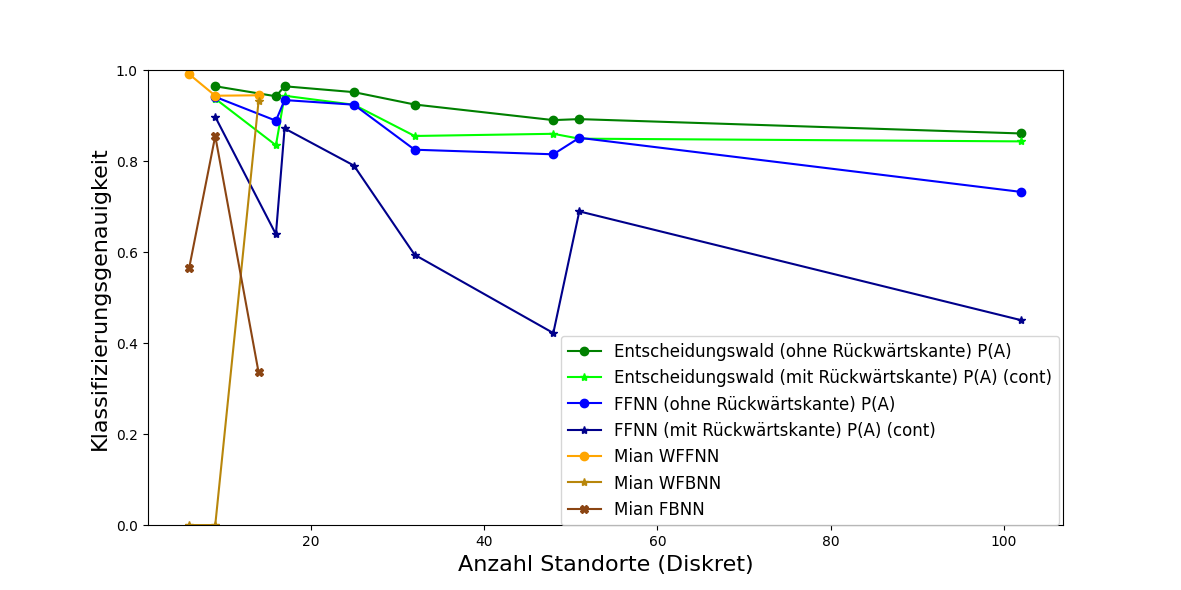
\includegraphics[width=\linewidth]{images/best_dt_vs_knn_fb_vs_no_fb.png}
    \caption{Die besten Klassifizierungsgenauigkeiten von ML-Modell mit und ohne Rückwärtskante und Mians Modelle über Standortkomplexitäten.}
    \label{fig:best_dt_vs_knn_fb_vs_no_fb}
\end{figure}
\newline
\newline
Mian kodierte in seinem Ansatz die Kanten als Standorte, was sich von den in dieser Arbeit benutzten Ansätzen unterscheidet.
Die in dieser Arbeit evaluierten Standortkomplexitäten, die Mians Evaluation am nächsten kommen, sind 16, mit dem Kodierungsansatz, der Kanten und Knoten kodiert,
und 17, mit dem Kodierungsansatz, der nur Knoten kodiert.
\newline
\newline
Aus Tabelle \ref{tab:predictions_by_acc_cont} können die Klassifizierungsergebnisse $P(A)_{\text{cont}}$ für die ML-Modelle mit Rückwärtskante entnommen werden
und aus Tabelle \ref{tab:predictions_wo_feedback_edge_by_acc} die Klassifizierungsergebnisse $P(A)$ für die ML-Modelle ohen Rückwärtskante.
Der beste Entscheidungswald mit Rückwärtskante bei einer Standortkomplexität von 16 Orten hat eine Klassifizierungsgenauigkeit $P(A)_{\text{cont}}$ von 83,52\% erzielt.
Das ist 9,74 Prozentpunkte schlechter als Mians WFBNN.
Das beste FFNN ist 29,32 Prozentpunkte schlechter.
Von der Modellstruktur her, ist das FBNN von Mian, der in dieser Arbeit verwendeten Struktur am ähnlichsten.
Im Vergleich mit diesem Modell ist der Entscheidungswald 49,95 Prozentpunkte besser und das FFNN 30,37 Prozentpunkte besser.
\newline
\newline
Der beste Entscheidungswald mit Rückwärtskante bei einer Standortkomplexität von 17 Orten ist 1,15 Prozentpunkte besser als Mians WFBNN.
Das beste FFNN ist 6,04 Prozentpunkte schlechter.
Im Vergleich mit Mians FBNN ist der Entscheidungswald 60,84 Prozentpunkte besser und das FFNN 53,65 Prozentpunkte besser.
\newline
\newline
Der beste Entscheidungswald ohne Rückwärtskante bei einer Standortkomplexität von 16 Orten ist 0,22 Prozentpunkte schlechter als Mians WFFNN.
Das beste FFNN ist 5,59 Prozentpunkte schlechter.
Bei einer Standortkomplexität von 17 Orten ist der beste Entscheidungswald 1,98 Prozentpunkte besser und das beste FFNN ist 1,05 Prozentpunkte schlechter.
Anzumerken ist, dass die Standortkomplexität in Vergleich zu Mian höher ist.
Außerdem wird kein Sensorengedächtnis verwendet, wodurch die ML-Modelle deutlich weniger Features nutzen und kleiner sind.

\subsection{Einfluss der Standortkomplexität}
ML-Modelle sind besser vergleichbar, wenn toleriert wird, dass das ML-Modell den Standort etwas zu früh betritt oder etwas zu spät verlässt,
solange es kontinuierlich den selben Standort angibt, da bei den Übergängen zwischen Standorten nicht immer eindeutig ein Standort bestimmt werden kann.
Tabellen \ref{tab:predictions_by_acc_5_cont} und \ref{tab:predictions_by_acc_5_wo_fb} geben diese Klassifizierungsgenauigkeit an,
wobei bis zu fünf fehlerhafte Klassifizierungen toleriert werden.
\newline
\newline
Abbildung \ref{fig:best_dt_vs_knn_pb_5_vs_pb_5_cont} vergleicht die ML-Modelle mit und ohne Rückwärtskante mit der Metrik $P(B\leq5)$.
Die Entscheidungswälder skalieren besser als die FFNNs mit steigender Standortkomplexität.
Wenn man eine lineare Regression über diese Klassifizierungsergebnisse legt,
verringert sich die Klassifizierungsgenauigkeit mit jedem zusätzlichen Standort bei den Entscheidungswäldern mit Rückwärtskante um 0,13 Prozentpunkte,
bei Entscheidungswäldern ohne Rückwärtskante um 0,1 Prozentpunkte,
bei FFNNs mit Rückwärtskante um 0,47 Prozentpunkte und bei FFNNs ohne Rückwärtskante um 0,24 Prozentpunkte.
\begin{figure}[h!]
    \centering
    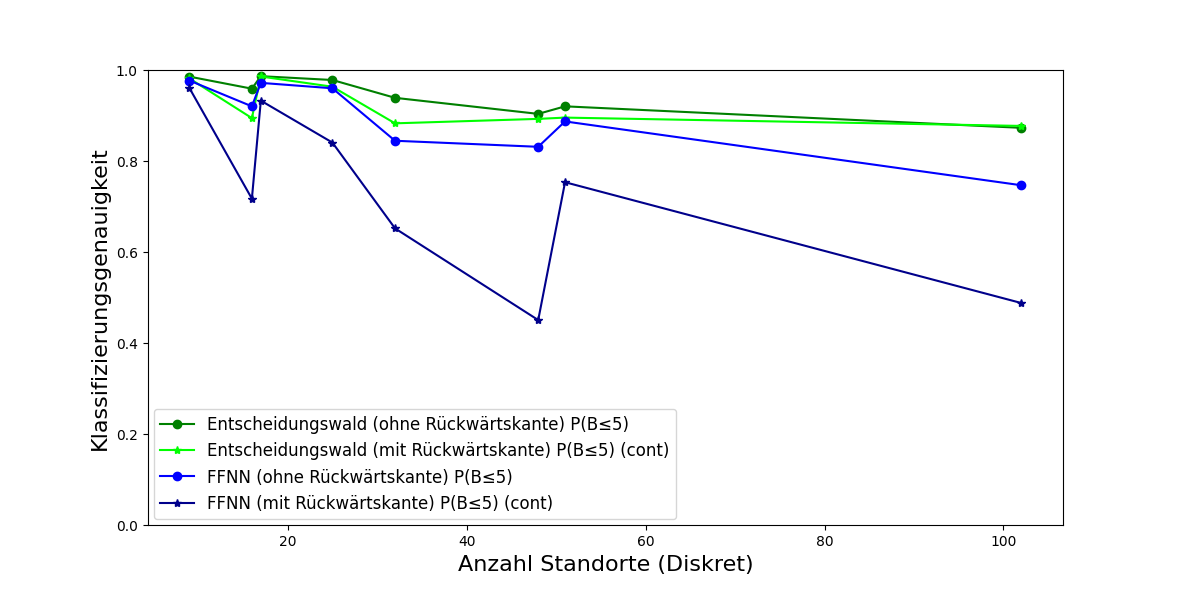
\includegraphics[width=\linewidth]{images/best_dt_vs_knn_pb_5_vs_pb_5_cont.png}
    \caption{Die besten Klassifizierungsgenauigkeiten $P(B\leq5)$ von ML-Modell mit und ohne Rückwärtskante über Standortkomplexitäten.}
    \label{fig:best_dt_vs_knn_pb_5_vs_pb_5_cont}
\end{figure}
\newline
\newline
Sowohl bei den Entscheidungswäldern, als auch bei den FFNNs, ist eine geringere Klassifizierungsgenauigkeit mit dem Kodierungsansatz, der Kanten und Knoten kodiert,
zu beobachten, als mit dem Kodierungsansatz, der nur die Knoten kodiert.
Insbesondere zwischen den Standortkomplexitäten 16 und 17, sowie 32, 48 und 52 ist diese Diskrepanz zu erkennen.
Aus diesem Grund ist zu schließen, dass der Kodierungsansatz, der nur Knoten kodiert, besser skaliert, als der Kodierungsansatz, der Kanten und Knoten kodiert.

\subsection{Einfluss der Hyperparameter}
Abbildungen \ref{fig:multiple_best_by_group_dt_max_depth_acc_5_cont} und \ref{fig:multiple_best_by_group_dt_max_depth_acc_5} zeigen, dass sich
als beste maximale Baumhöhe hat sich 16 herausgestellt, wobei 32 und 64 marginal schlechtere Ergebnisse erzielten.
Eine maximale Baumhöhe von 8 war nicht ausreichend, da es für hohe Standortkomplexitäten schlechtere Ergebnisse erzielt hat.
Bei gleicher Waldgröße haben die maximalen Baumhöhen von 32 und 64 äquivalente Ergebnisse erzielt für Entscheidungswälder mit Rückwärtskante.
\newline
\newline
Dies schließt aber nicht aus, dass andere Szenarien nicht von größeren maximalen Baumhöhen profitieren könnten.
Abbildungen \ref{fig:multiple_best_by_group_dt_trees_acc_5_cont} und \ref{fig:multiple_best_by_group_dt_trees_acc_5} zeigen
die Klassifizierungsergebnisse von Entscheidungswäldern verschiedener Waldgröße.
Eine Waldgröße von 8 hat nur marginal schlechtere Ergebnisse bei 102 Standorten erzielt, als die Waldgrößen 16, 32 und 64.
Aus diesem Grund ist eine Waldgröße von 8 ausreichend, oder könnte womöglich reduziert werden.
\newline
\newline
Die FFNNs mit Rückwärtskante verhalten sich sehr volatil (Abbildungen \ref{fig:multiple_best_by_group_knn_layers_acc_5_cont}
und \ref{fig:multiple_best_by_group_knn_neurons_acc_5_cont}), weswegen keine Aussage darüber getroffen werden kann.
Die FFNNs ohne Rückwärtskante erzielen konsistentere Ergebnisse.
Abbildung \ref{fig:multiple_best_by_group_knn_layers_acc_5} zeigt, dass die Klassifizierungsergebnisse
für verschiedene Anzahlen von verdeckten Schichten sich nicht stark voneinander unterscheiden.
Zwei verdeckte Schichten haben sich insgesamt marginal besser erwiesen als eine, vier und acht verdeckte Schichten,
aber die zusätzliche Klassifizierungsgenauigkeit müsste mit der zusätzlichen Größe des FFNNs abgewogen werden.
Abbildung \ref{fig:multiple_best_by_group_knn_neurons_acc_5} zeigt, dass die Klassifizierungsgenauigkeit
mit steigender Anzahl von Neuronen in der verdeckten Schicht skaliert.
Auch hier müsste die gewonnene Klassifizierungsgenauigkeit mit der zusätzlichen Größe des FFNNs abgewogen werden.
